\graphicspath{{exp_design/fig/}}
{
\tikzset{external/figure name/.add={exp_design/}{}}

\chapter{Experimental design} \label{chap:exp_design}

    \paragraph
    As discussed in Chapter~\ref{chap:lit_study}, experimental data is a valuable part of any study involving multirotors control.
    This chapter will provide an overview of the hardware components, software toolchain, HITL simulations, and practical methodology used in this work.

    \FloatBarrier\section{Hardware components}

        \paragraph
        The hardware involved in this work includes a multirotor vehicle, a payload angle sensor, and an \gls{OBC}.
        These hardware elements are coupled together into the final multirotor system which will be used for practical flights.

        \FloatBarrier\subsection{Multirotor}

            \begin{figure}[ht]
                \centering
                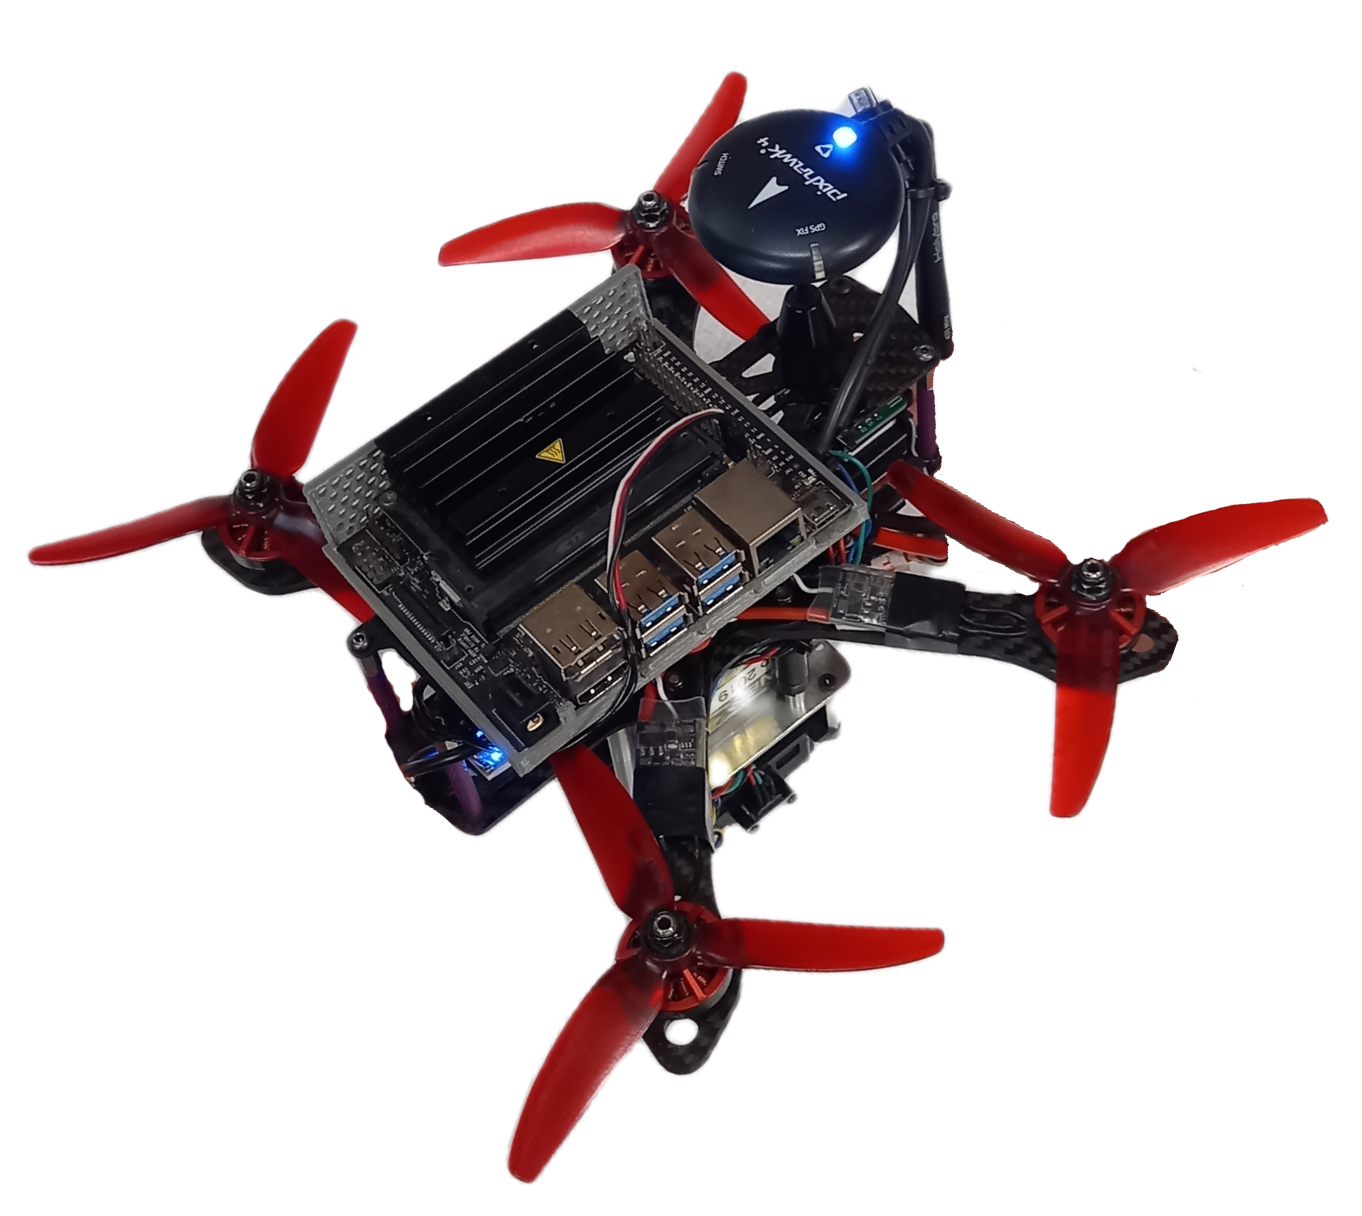
\includegraphics[width=0.5\linewidth]{exp_design/fig/honeybee}
                \caption{Honeybee quadrotor equipped with a \gls{OBC} and payload angle sensor}
                \label{fig:honeybee}
            \end{figure}

            \paragraph
            The multirotor used in this work is a lightweight and modular quadrotor named \emph{Honeybee} which was developed in the \gls{ESL} at Stellenbosch University \cite{Grobler2020}.
            Figure~\ref{fig:honeybee} shows an photo of Honeybee equipped with an \gls{OBC} and payload angle sensor.
            Table~\ref{tbl:honeybee_specs} summarises the physical parameters of this multirotor system.
            Note that the mass and inertial parameters include the \gls{OBC} and payload angle sensor.
            The thrust profile of each motor is given by the third-order polynomial mapping the input \gls{PWM} signal, $x$, to the thrust output, $T_m$:
            \begin{equation}
                T_m(x) = -3.508 \cdot 10^{-9} x^3 + 1.627 \cdot 10^{5} x^2 - 0.0172 x + 4.528
            \end{equation}

            \begin{table}[!h]
                \renewcommand{\arraystretch}{1.1}
                \centering
                \caption{Physical parameters of Honeybee.}
                \begin{tabularx}{0.9\linewidth}{@{}lll@{}}
                    \toprule
                    \textbf{Description} & \textbf{Parameter} & \textbf{Value} \\
                    \midrule
                    Mass                        & $m_Q$     & 0.952~kg \\
                    Motor distance              & $d$       & 0.11~m \\
                    Virtual yaw moment arm      & $R_N$     & $7.997 \cdot 10^{-3}$~m \\
                    Motor time constant         & $\tau$    & 15~ms \\
                    Mass moment of inertia about $\bm{\bar{x}}_\mathcal{B}$                 & $I_{xx}$      & $2.00 \cdot 10^{-3}$~kg$\cdot$m$^2$ \\
                    Mass moment of inertia about $\bm{\bar{y}}_\mathcal{B}$                 & $I_{yy}$      & $1.32 \cdot 10^{-3}$~kg$\cdot$m$^2$ \\
                    Mass moment of inertia about $\bm{\bar{z}}_\mathcal{B}$                 & $I_{zz}$      & $3.35 \cdot 10^{-3}$~kg$\cdot$m$^2$ \\
                    Aerodynamic drag coefficient in $\bm{\bar{x}}_\mathcal{B}$ direction    & $C_{Q_X}$     & 0.096~m$^2$ \\	
                    Aerodynamic drag coefficient in $\bm{\bar{y}}_\mathcal{B}$ direction    & $C_{Q_Y}$     & 0.096~m$^2$ \\	
                    Aerodynamic drag coefficient in $\bm{\bar{z}}_\mathcal{B}$ direction    & $C_{Q_Z}$     & 0.256~m$^2$ \\	
                    \bottomrule
                \end{tabularx}
                \label{tbl:honeybee_specs}
            \end{table}
        
            \paragraph
            The \gls{FC} implemented on Honeybee is a \emph{Pixhawk 4 mini} which runs the flight stack firmware.
            Figure~\ref{fig:pixhawk} shows what the Pixhawk 4 mini looks like.
            This board includes internal \gls{IMU}, magnetometer, and barometer sensors and is connected to an external \gls{GPS} sensor and an additional magnetometer.
            Furthermore, an \gls{RC} receiver is used to communicate with a radio transmitter for manual pilot control and a telemetry radio module is used for communication with a ground control station.
            The \gls{OBC} and external payload angle sensors are also connected to the \gls{FC}.

            \begin{figure}[ht]
                \centering
                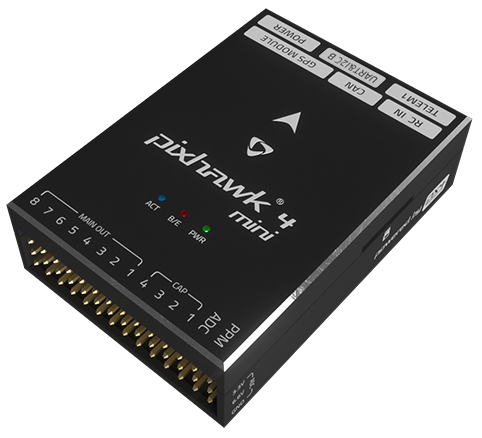
\includegraphics[width=0.3\linewidth]{exp_design/fig/pixhawk}
                \caption{Photo of a Pixhawk 4 mini \gls{FC} \cite{PX4userguide}}
                \label{fig:pixhawk}
            \end{figure}
            
        \FloatBarrier\subsection{Payload angle sensor}

            \paragraph
            A sensor is required to measure the payload state as Euler angles about the $\bm{\bar{x}}_\mathcal{B}$ and $\bm{\bar{y}}_\mathcal{B}$ axes.
            Figure~\ref{fig:payload_state_sensor} shows a customised sensor attached to the Honeybee airframe for this purpose.
            
            \begin{figure}[ht]
                \centering
                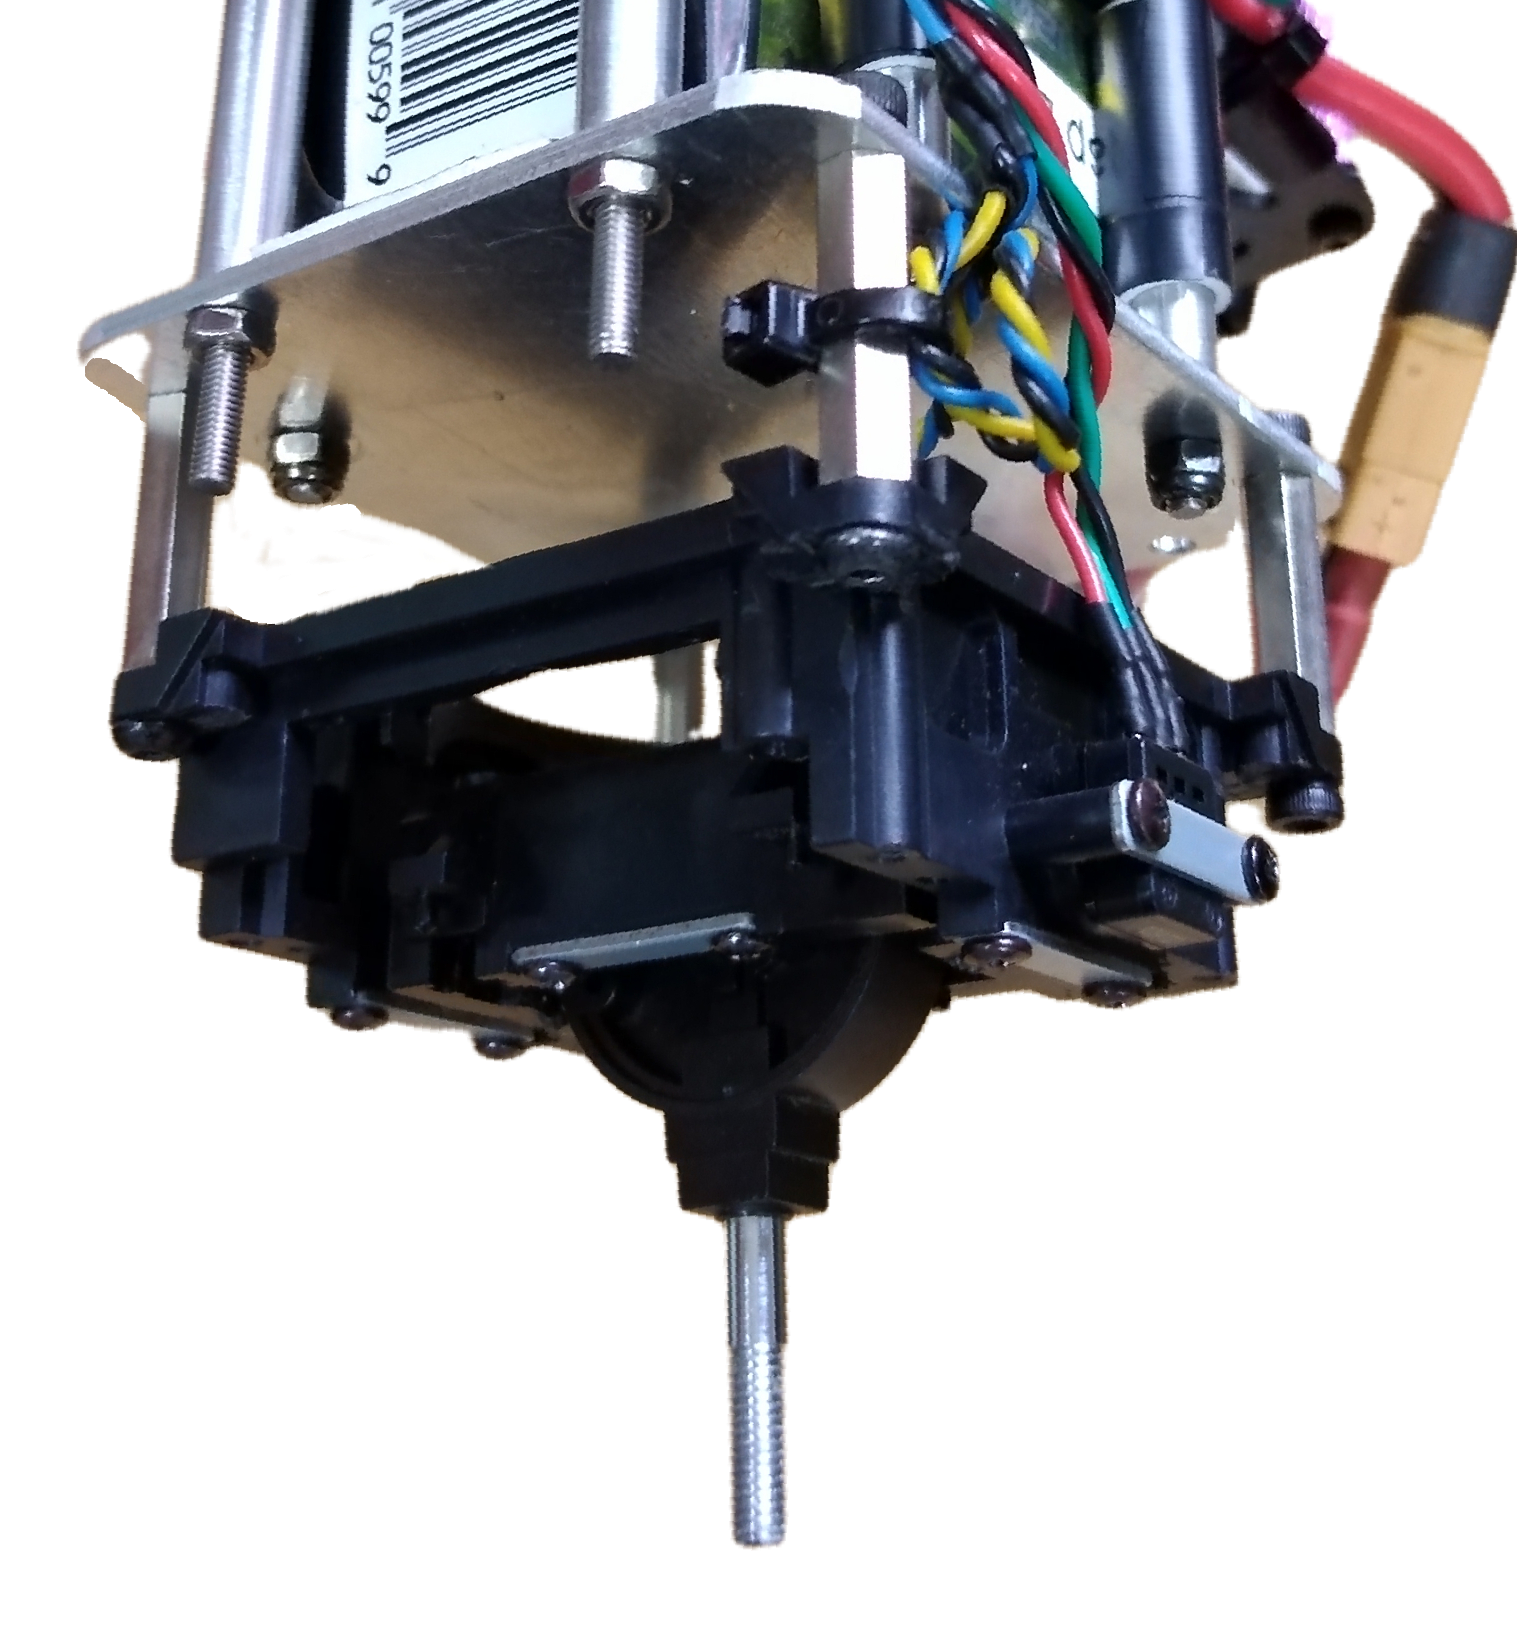
\includegraphics[width=0.3\linewidth]{exp_design/fig/payload_state_sensor}
                \caption{Payload angle sensor with linear potentiometers}
                \label{fig:payload_state_sensor}
            \end{figure}

            \paragraph
            This sensor was constructed from a two-axis joy-stick and two linear potentiometers.
            Each potentiometer is implemented as a voltage divider and attached to an \gls{ADC} channel on the \gls{FC}. 
            An experiment was performed to map the \gls{ADC} reading to an angle measurement with a straight line function, which is implemented on the \gls{FC}.
            A cable can then be attached to this device to transport a suspended payload and measure the swing angles during flight.

        \FloatBarrier\subsection{On-Board Computer}

            \paragraph
            An \gls{OBC}, also called a companion computer, is used to run intensive computational processes that cannot be handled by the \gls{FC}.
            A NVIDIA\textsuperscript{\textregistered} Jetson Nano\texttrademark, shown in Figure~\ref{fig:jetson}, is used as the \gls{OBC} for Honeybee.
            This has 4GB memory and a quad-core processor which runs at 1.43 GHz.
            The \gls{OBC} is connected to a serial port on the \gls{FC} for communication.

            \begin{figure}[ht]
                \centering
                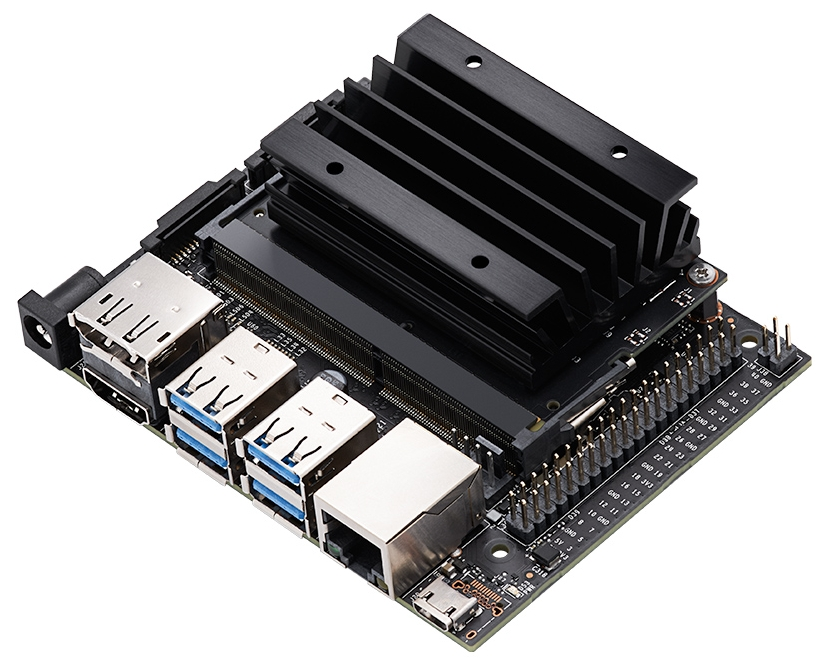
\includegraphics[width=0.3\linewidth]{exp_design/fig/jetson}
                \caption{NVIDIA\textsuperscript{\textregistered} Jetson Nano\texttrademark~\cite{NVIDIA} used as a \gls{OBC}}
                \label{fig:jetson}
            \end{figure}
            
    \FloatBarrier\section{Software Toolchain}

        \paragraph
        The software toolchain used with Honeybee includes PX4-Autopilot, \gls{ROS}, and Gazebo simulator.
        This is a popular toolchain applied in research and was also used and described by \citet{Erasmus2020}, \citet{Slabber2020}, and \citet{Grobler2020}.
        A brief overview of the software toolchain is provided here.
        % MATLAB/Simulink was also used to generate standalone \gls{ROS} nodes which runs on the \gls{OBC}.

        \FloatBarrier\subsection{PX4-Autopilot}

            \paragraph
            PX4-Autopilot is an open-source flight stack that focuses on autonomous \glspl{UAV} \cite{Meier2015}.
            This is a popular flight stack used in research and industry applications.
            \gls{SITL} and \gls{HITL} simulations are supported by PX4, which is helpful for research and development purposes.
            
            \paragraph
            \gls{QGC} is the recommended ground station software for PX4 systems.
            A ground station computer running \gls{QGC} can be used to monitor and control a PX4 vehicle.
            \gls{QGC} communicates with PX4 via the MAVLink protocol over a telemetry connection during practical flights.
            \gls{QGC} is also an open-source product.
            
        \FloatBarrier\subsection{Gazebo simulator}

            \paragraph
            Gazebo is an open-source graphical-based physics simulator used for robotics and is the recommended simulator in the PX4 development toolchain \cite{PX4userguide}.
            This simulator is capable of both \gls{SITL} and \gls{HITL} simulations.
            The PX4 flight stack includes quadrotor models developed for Gazebo which include realistic sensor plugins.
            These plugins apply sensor noise, drift and bias which replicates the actual sensors used on Pixhawk boards.
            The physical parameters of these models were changed to match Honeybee and a suspended payload was added to the model as shown in Figure~\ref{fig:gazebo_model}.

            % \begin{figure}[ht]
            %     \centering
            %     \includegraphics[width=0.6\linewidth]{exp_design/fig/gazebo_model}
            %     \caption{Model of Honeybee in Gazebo simulator}
            %     \label{fig:gazebo_model}
            % \end{figure}

        \FloatBarrier\subsection{Robot Operating System}

            \paragraph
            \gls{ROS} is a communication framework with a set of tools used for robotics and control applications \cite{Quigley2009}. 
            \gls{ROS} is open-source and is supported by PX4.
            In this architecture, executables are called \gls{ROS} nodes and communicate with each other using messages in a publish-subscribe architecture.
            A ROS node can publish messages to a topic, and a different node can subscribe to that topic to read those messages.

            \paragraph
            MAVROS is a open-source ROS package which provides a bridge between ROS and PX4 through the MAVLink protocol.
            \gls{QGC} and Gazebo also communicate with PX4 through MAVLink.
            A MAVROS node receives MAVLink messages from PX4 and converts this to published ROS topics for other ROS nodes to access.
            The MAVROS node also subscribes to topics to receive ROS messages and send this data to PX4. 

            % \begin{figure}[ht]
            %     \centering
            %     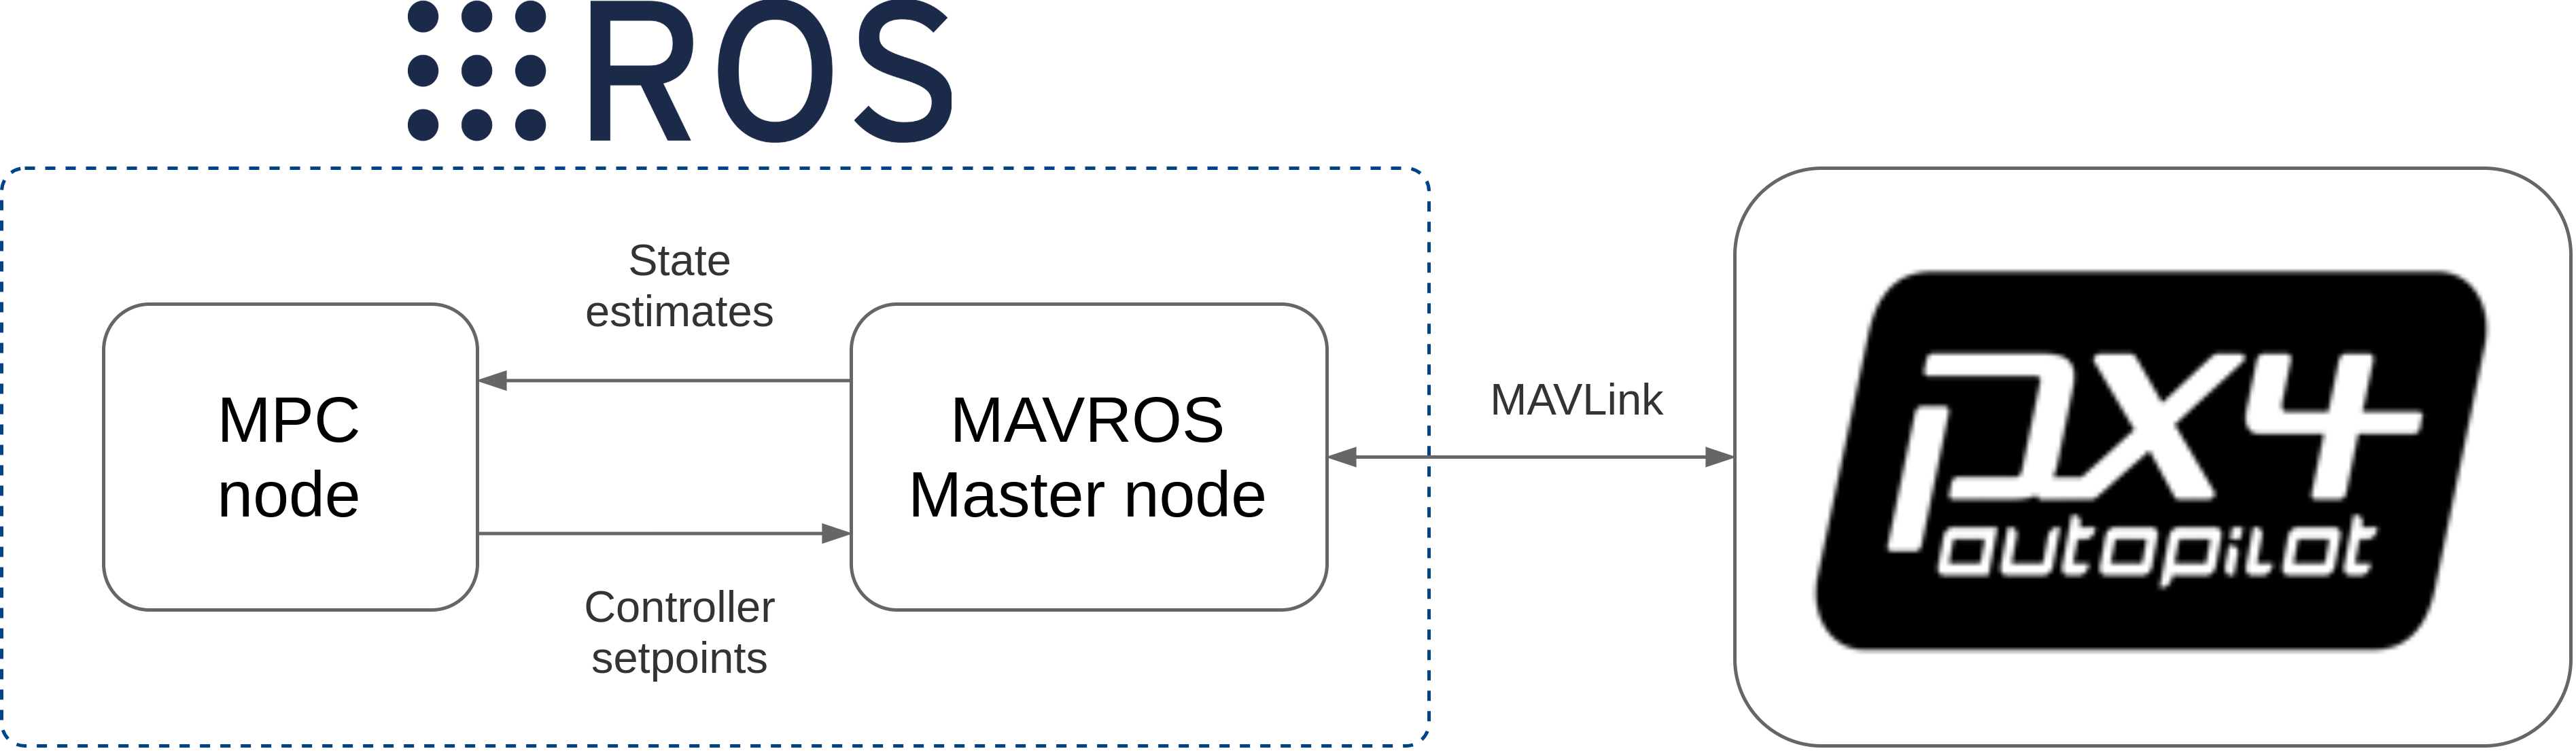
\includegraphics[width=0.6\linewidth]{exp_design/fig/MAVROS}
            %     \caption{Communication between \gls{ROS}, flight stack, simulator, and ground station \cite{Grobler2020}}
            %     \label{fig:MAVROS}
            % \end{figure}

            % ?? Illustrate MAVROS

            \paragraph
            Figure~\ref{fig:MAVROS}

            MATLAB/Simulink generate nodes

    \FloatBarrier\section{Hardware-in-the-Loop simulations} \label{sec:exp_design_hitl}

        \paragraph
        MATLAB is used to generate an \gls{MPC} \gls{ROS} node 
        This \gls{ROS} node receives state feedback from the Gazebo simulator,
        computes the optimal control action,
        and sends the setpoint to PX4 through the package 'mavros'.

    \FloatBarrier\section{Practical flights}
        
        \paragraph
        As discussed in Chapter~\ref{chap:system_id}, 
        generating data for the parameter estimation techniques involves two distinct flight stages.
        Firstly, the multirotor hovers with the suspended payload to gather data for payload mass estimation.
        A velocity step setpoint is then commanded to stimulate the swinging payload system for cable length estimation.
        Hence, the same methodology used for simulations will be used for practical flights.

        \paragraph
        For the data-driven techniques, the generation of practical training and testing data
        also follows the same general methodology as simulated flights:
        \begin{enumerate}
            \item Data logging starts when the multirotor is armed
            \item Takeoff and hover with the multirotor
            \item Command velocity step setpoints
            \item Land the multirotor
            \item Data logging stops when the multirotor is disarmed
            \item Download the data log from the multirotor
            \item Split the data into separate training and testing periods
            \item Build a model from the training data
            \item Perform model predictions over the testing data to calculate an error metric
        \end{enumerate}

        \paragraph
        Figure~\ref{fig:honeybee_with_payload} shows the Honeybee multirotor with a suspended payload during a practical flight.
        Numerous flights were performed with different 
        payload masses, 
        cable lengths, 
        wind conditions, 
        and dynamic payloads.
        The system identification methods were then performed for these different use cases.
        
        \paragraph
        The major differences between the simulated and practical flights involve the attachment of the payload and wind disturbances.
        In simulations, the payload cable is attached to the exact \gls{CoM} of the multirotor.
        However, for practical flights the cable is attached slightly below the \gls{CoM} of Honeybee due to mechanical constraints.
        Practical flights are also influenced by wind disturbances which were not considered in simulations.
        The measurement noise experienced by a practical multirotor may also differ from the noise models used in simulations.

        \begin{figure}[!htb]
            \centering
            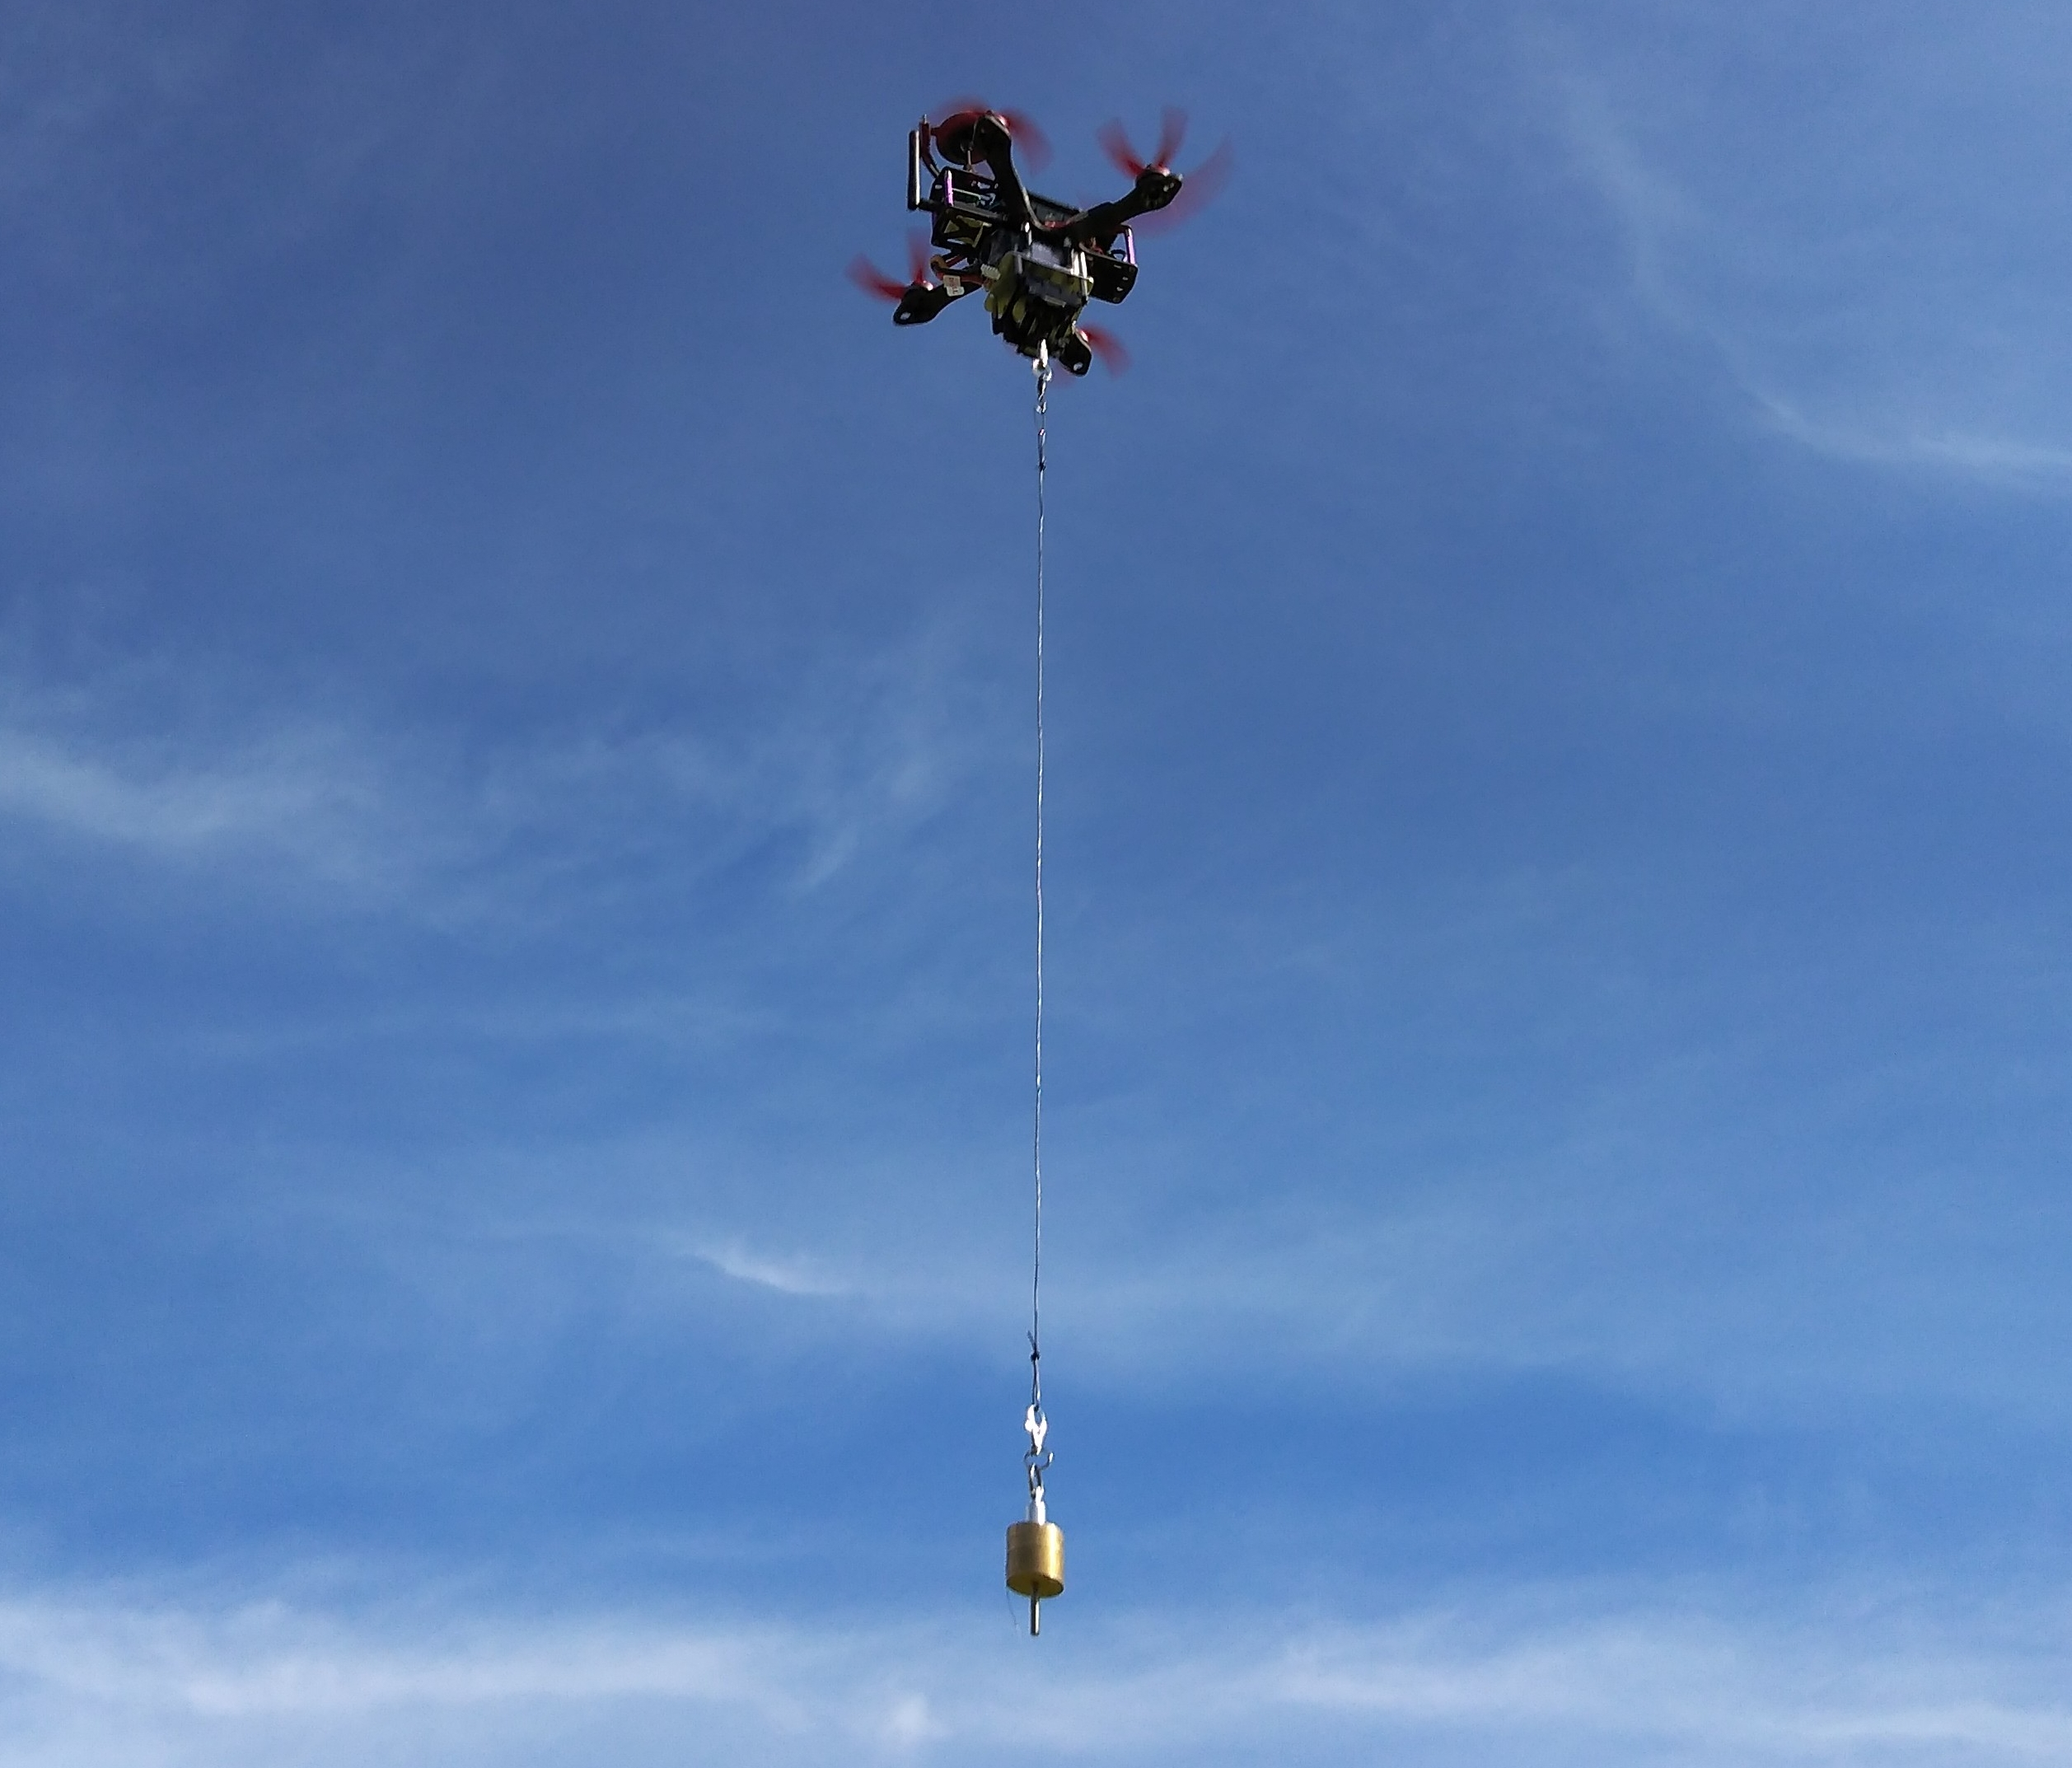
\includegraphics[width=0.5\linewidth]{honeybee_with_payload.jpg}
            \caption{Practical flight with Honeybee and a suspended payload}
            \label{fig:honeybee_with_payload}
        \end{figure}

    \FloatBarrier\section{Summary}

}
